\section{Đặt vấn đề}
\label{sec:problem}

\subsection{Giới thiệu chung về Tổng hợp ảnh đa phương thức}
\label{ssec:intro-mif}

Trong y học hiện đại, chẩn đoán chính xác đóng vai trò quyết định trong việc lựa chọn phác đồ điều trị, đặc biệt với các bệnh lý phức tạp như ung thư, đột quỵ và rối loạn thần kinh. Mỗi phương thức chụp ảnh y tế cung cấp một góc nhìn khác nhau về cơ thể người bệnh: chụp cắt lớp vi tính (CT) cho thấy rõ cấu trúc xương và mô đặc; chụp cộng hưởng từ (MRI) có độ phân giải cao đối với mô mềm; trong khi chụp cắt lớp phát xạ positron (PET) và chụp cắt lớp đơn photon (SPECT) cung cấp thông tin chức năng và chuyển hóa. Mỗi phương thức đều có ưu điểm và hạn chế riêng, buộc bác sĩ phải đối chiếu đồng thời nhiều loại ảnh trong quá trình chẩn đoán.

\textbf{Tổng hợp ảnh đa phương thức y tế} (Medical Image Fusion --- MIF) ra đời nhằm tự động kết hợp thông tin bổ sung từ hai phương thức ảnh thành một ảnh duy nhất, vừa giữ lại cấu trúc giải phẫu chi tiết, vừa thể hiện được thông tin chức năng. Một ảnh tổng hợp chất lượng cao giúp rút ngắn thời gian chẩn đoán, giảm sai sót và hỗ trợ ra quyết định lâm sàng nhanh hơn. Hình~\ref{fig:mif-examples} minh họa kết quả tổng hợp trên ba cặp modality phổ biến trong y học.

\begin{figure}[H]
    \centering
    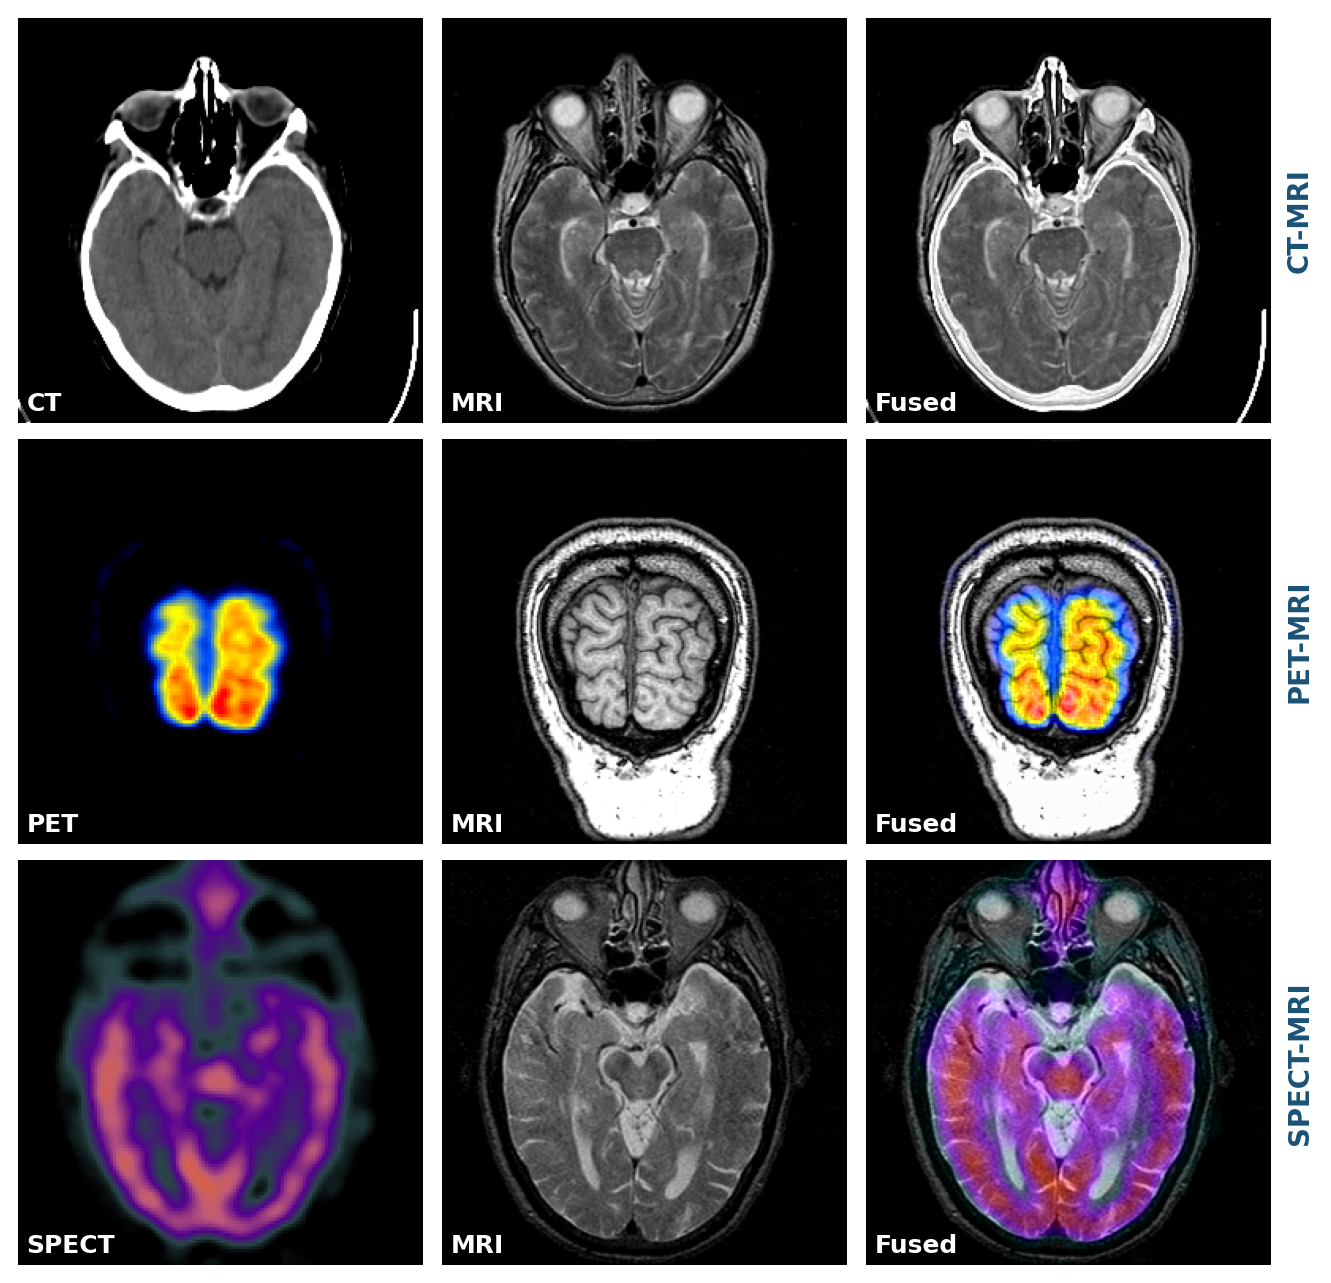
\includegraphics[width=0.57\textwidth]{figures/fig1_mif_examples.png}
    \caption{Minh họa bài toán tổng hợp ảnh đa phương thức y tế trên tập dữ liệu Harvard. Mỗi hàng trình bày một cặp modality: ảnh nguồn thứ nhất (CT/PET/SPECT), ảnh MRI tương ứng, và ảnh tổng hợp bởi CDDFuse.}
    \label{fig:mif-examples}
\end{figure}

\subsection{Thách thức về dữ liệu y tế}
\label{ssec:challenges}

Khác với các bài toán thị giác máy tính thông thường, tổng hợp ảnh y tế đối mặt với một thách thức cơ bản: \textbf{không tồn tại ảnh tổng hợp chuẩn} (ground-truth fused image) trong thực tế lâm sàng. Không có thiết bị y tế nào tạo ra trực tiếp ảnh kết hợp đồng thời thông tin CT và MRI tại cùng một thời điểm, do đó không thể xây dựng nhãn giám sát theo cách thông thường. Điều này đòi hỏi các phương pháp học sâu phải thiết kế hàm mất mát không cần nhãn, dựa trên các ràng buộc về bảo toàn thông tin và chất lượng thị giác.

Bên cạnh đó, dữ liệu ảnh y tế có tính phân bố không đồng nhất cao giữa các bệnh nhân, thiết bị và cơ sở y tế khác nhau, trong khi quy mô dataset thường nhỏ hơn nhiều so với các bài toán thị giác thông thường. Đây là những ràng buộc quan trọng định hướng thiết kế mô hình theo hướng \emph{nhẹ, hiệu quả tham số và không phụ thuộc vào nhãn đầu ra} (Hình~\ref{fig:no-gt}).

\begin{figure}[H]
    \centering
    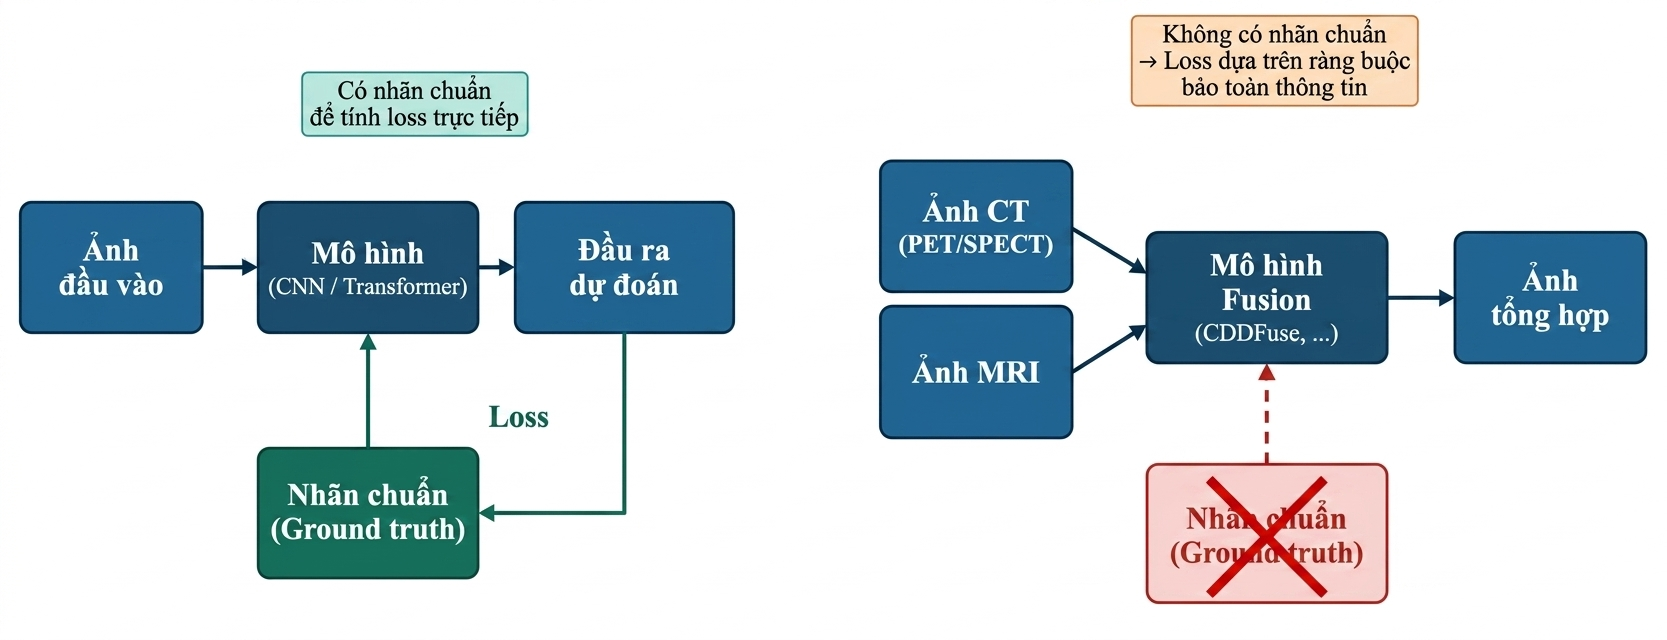
\includegraphics[width=\textwidth]{figures/fig2_no_groundtruth.png}
    \caption{So sánh paradigm học có giám sát (trái) và bài toán tổng hợp ảnh y tế (phải). Trong MIF, không tồn tại ảnh tổng hợp chuẩn làm nhãn giám sát, buộc các phương pháp phải thiết kế hàm mất mát dựa trên ràng buộc bảo toàn thông tin.}
    \label{fig:no-gt}
\end{figure}

Trong bối cảnh này, \textbf{CDDFuse}~\cite{zhao2023cddfuse} (CVPR 2023) là một phương pháp tiêu biểu, sử dụng kiến trúc dual-branch Transformer--CNN với cơ chế phân rã đặc trưng theo tương quan, đạt hiệu năng hàng đầu trên các benchmark MIF. Tuy nhiên, cả hai nhánh Base và Detail trong CDDFuse đều dùng \textbf{phép cộng đơn giản} $f_F = f_V + f_I$ làm quy tắc tổng hợp, không khai thác được sự khác biệt bản chất giữa thành phần cấu trúc toàn cục (Base) và thành phần chi tiết đặc trưng từng modality (Detail).

\section{Các nghiên cứu liên quan}
\label{sec:related}

Tổng hợp ảnh y tế đa phương thức đã phát triển qua bốn hướng tiếp cận chính:

\textbf{Phương pháp truyền thống.} Các kỹ thuật biến đổi đa tỉ lệ như Wavelet, Curvelet và biểu diễn thưa thớt (sparse representation)~\cite{liu2018survey} phân rã ảnh thành các thành phần tần số khác nhau, sau đó kết hợp theo quy tắc thiết kế thủ công như max-pooling hoặc trung bình có trọng số. Nhóm phương pháp này có cơ sở lý thuyết vững chắc nhưng phụ thuộc nặng vào đặc trưng thiết kế tay, khó khái quát hóa cho các cặp modality đa dạng trong y tế.

\textbf{Học biểu diễn (Representation Learning).} Các phương pháp học đặc trưng không giám sát như Autoencoder và Variational Autoencoder học cách nén và tái tạo ảnh từ không gian tiềm ẩn. DenseFuse~\cite{li2019densefuse} và NestFuse áp dụng kiến trúc Encoder--Decoder dựa trên DenseNet, huấn luyện qua hàm mất mát tái tạo không cần nhãn, cho phép trích xuất đặc trưng giàu ngữ nghĩa hơn so với phương pháp truyền thống.

\textbf{Học sâu với CNN, Attention và Transformer.} Sự phát triển của mạng tích chập và cơ chế chú ý đã thúc đẩy thế hệ phương pháp mạnh hơn, học trực tiếp quy tắc tổng hợp từ dữ liệu. U2Fusion và RFN-Nest khai thác kiến trúc đa tỉ lệ với cơ chế attention để tập trung vào vùng thông tin quan trọng. Sự ra đời của Transformer mở rộng khả năng nắm bắt phụ thuộc tầm xa: CDDFuse~\cite{zhao2023cddfuse} kết hợp Restormer Encoder với Invertible Neural Network để phân rã đặc trưng thành nhánh Base và Detail; APGFusion~\cite{hu2024apgfusion} bổ sung cơ chế Adaptive Pooling Guided cải thiện tổng hợp thông tin không gian đa tỉ lệ.

\textbf{Mô hình sinh (Generative AI).} Hướng mới nhất ứng dụng Diffusion Model và Foundation Model vào bài toán MIF. Các phương pháp dựa trên Diffusion như DDFM mô hình hóa quá trình tổng hợp như một bài toán suy diễn xác suất, tạo ra ảnh tổng hợp chất lượng cao về mặt thị giác. Foundation Model với pretrained trên dữ liệu lớn mở ra hướng transfer learning cho y tế, tuy nhiên chi phí tính toán và yêu cầu dữ liệu lớn vẫn là rào cản thực tiễn.

Mặc dù có nhiều cải tiến theo từng hướng, hầu hết các phương pháp vẫn áp dụng quy tắc tổng hợp đối xứng cho mọi thành phần đặc trưng. Tác động của việc thiết kế \emph{quy tắc tổng hợp bất đối xứng} --- khác nhau cho nhánh Base và Detail --- chưa được khảo sát có hệ thống. Đây chính là khoảng trống mà đồ án hướng đến.

\section{Mục tiêu và Đóng góp của Đồ án}
\label{sec:goal}

Mục tiêu cốt lõi của đồ án là đề xuất mô hình \textbf{CDDFuse-AG} nhằm cải thiện chất lượng tổng hợp ảnh y tế đa phương thức thông qua thiết kế lại quy tắc tổng hợp đặc trưng theo hướng bất đối xứng, mà không thay đổi kiến trúc Encoder--Decoder đã được pretrained. Đồ án hướng tới việc khắc phục hạn chế cốt lõi của CDDFuse gốc --- áp dụng cùng một phép cộng đơn giản cho cả hai nhánh Base và Detail --- đồng thời đảm bảo so sánh công bằng và tiết kiệm tài nguyên tính toán thông qua việc tái sử dụng toàn bộ backbone đã huấn luyện.

Để hiện thực hóa mục tiêu này, đồ án lựa chọn hướng tiếp cận khảo sát thực nghiệm có kiểm soát theo chiến lược \emph{one-factor-at-a-time ablation} ba giai đoạn. Ở giai đoạn khảo sát quy tắc tổng hợp Cơ sở, năm quy tắc thay thế được thiết kế và đánh giá cho nhánh Base trong khi cố định nhánh Detail theo paper gốc. Ở giai đoạn khảo sát quy tắc Chi tiết, tám quy tắc được khảo sát tương tự cho nhánh Detail với nhánh Base cố định. Các quy tắc tốt nhất từ hai giai đoạn sau đó được kết hợp bất đối xứng (Base rule $\neq$ Detail rule) để tạo ra mô hình CDDFuse-AG cuối cùng. Toàn bộ thực nghiệm được đánh giá trên tập \emph{Harvard Medical Image Fusion} với 22 chỉ số chất lượng theo chuẩn VIFB~\cite{liu2020vifb} và xếp hạng tổng hợp bằng phương pháp Composite Z-score.

Các đóng góp chính của đồ án được tóm tắt như sau:

\begin{itemize}\itemsep4pt
    \item Đề xuất chiến lược thực nghiệm ablation ba giai đoạn có kiểm soát, khảo sát hệ thống 13 quy tắc tổng hợp (5 quy tắc Base và 8 quy tắc Detail), bao phủ từ phương pháp truyền thống (L1-norm, SML, SF, VSM) đến học sâu (Adaptive Gating, Saliency Gate, Soft PCNN), cung cấp cơ sở thực nghiệm toàn diện cho bài toán lựa chọn fusion rule trong MIF.

    \item Đề xuất mô hình \textbf{Comb-WAvg-SML (CDDFuse-AG)}: thiết kế bất đối xứng với Weighted Average Scalar cho nhánh Base và Sum-Modified-Laplacian cho nhánh Detail, chỉ bổ sung $\sim 8.200$ tham số fusion nhưng vượt CDDFuse rõ rệt trên CT-MRI (composite z-score $+0{,}240$ so với $-0{,}483$, chênh $+0{,}723$).

\end{itemize}

\section{Bố cục đồ án}
\label{sec:outline}

Phần còn lại của đồ án tốt nghiệp được tổ chức thành năm chương, cụ thể như sau:

\begin{itemize}\itemsep4pt
    \item \textbf{Chương~\ref{ch:background} --- Cơ sở lý thuyết.} Trình bày các nền tảng lý thuyết liên quan đến bài toán tổng hợp ảnh y tế đa phương thức, bao gồm kiến trúc dual-branch Transformer--CNN của CDDFuse, cơ chế phân rã đặc trưng Base/Detail, các phương pháp tổng hợp đặc trưng truyền thống và chỉ số đánh giá chất lượng ảnh tổng hợp.

    \item \textbf{Chương~\ref{ch:method} --- Phương pháp đề xuất.} Mô tả chi tiết chiến lược thực nghiệm ablation ba giai đoạn có kiểm soát, công thức toán học của 13 quy tắc tổng hợp được khảo sát và thiết kế mô hình bất đối xứng Comb-WAvg-SML. Trọng tâm của chương là lý giải lý do chọn quy tắc riêng biệt cho nhánh Base và nhánh Detail.

    \item \textbf{Chương~\ref{ch:results} --- Thí nghiệm và kết quả.} Trình bày thiết lập thực nghiệm, kết quả đánh giá định lượng với bảng Composite Z-score cho cả ba giai đoạn và phân tích chi tiết theo từng modality CT/PET/SPECT.

    \item \textbf{Chương~\ref{ch:discussion} --- Thảo luận.} Phân tích và lý giải các phát hiện thực nghiệm, bao gồm hiện tượng Modality-Specificity, vai trò của thiết kế bất đối xứng, hạn chế của đồ án và so sánh với phương pháp SOTA APGFusion 2024.

    \item \textbf{Chương~\ref{ch:conclusion} --- Kết luận và hướng phát triển.} Tổng kết các kết quả và đóng góp chính của đồ án, đồng thời đề xuất các hướng nghiên cứu mở rộng trong tương lai.
\end{itemize}

Tóm lại, Chương~1 đã giới thiệu bài toán tổng hợp ảnh y tế đa phương thức cùng hạn chế của CDDFuse trong thiết kế quy tắc tổng hợp đối xứng, từ đó xác định mục tiêu và định hướng xây dựng mô hình CDDFuse-AG. Trên cơ sở đó, Chương~\ref{ch:background} tiếp theo sẽ trình bày chi tiết các nền tảng lý thuyết và công cụ cần thiết cho việc thiết kế và triển khai phương pháp đề xuất.
